\documentclass[psfig,preprint]{aastex}
%\documentstyle[12pt,aasms4]{article}
%\documentstyle[11pt,aaspp4]{article}
%\documentstyle[aas2pp4]{article}
\begin{document}
 
\title{SPECIFIC INTENSITY: THE FOUNT OF ALL KNOWLEDGE! \\ or\dots \\
{\boldmath $I, \ T_B, \ T_{SYS}, \ T_{RCVR}, \ S,$ and $\tau
\Delta \nu$}}


\author{ Carl Heiles \ \today} 

\section {INTRODUCTION}

	The cosmic radiation that we measure differs from radiation
produced by humankind.   Humankind's transmitters usually produce
radiation at specific frequencies; this radiation is modulated with an
information-containing signal of some sort, such as rap music (here we
use the term ``information'' loosely).  In contrast, cosmic radiation is
not produced by slow modulation of a carrier frequency with an
information-containing signal generated by an intelligent being. 
Rather, cosmic radiation is produced by random processes, of which there
are three common types: collisions between electrons and protons in a
gas at temperature $T$; spiraling of relativistic electrons in a
magnetic field; and transitions between energy levels of an atom or
molecule.  The former two generate radiation over a wide spectrum of
frequencies while the latter generates a narrow spectrum called a {\it
spectral line}.  The radiation from the former two is called {\it
continuum radiation} because its frequency spectrum is very broad and
featureless.  For these random processes, we can describe the spectrum
as a sum of Fourier components; all frequency components in a small
bandwidth have comparable power and random electrical phases, and the
total power varies with frequency to give the spectrum we observe.

	Continuum radiation is produced by all astronomical objects. 
For example, stars produce continuum radiation that is strongest at
optical or IR frequencies.  Galaxies and clouds of hot gas also produce
optical and IR continuum radiation.  They also produce continuum
radiation at radio frequencies, and this is usually much less intense
than the optical continuum radiation. Some sources have relativistic
electrons, and these sometimes produce powerful radiation at radio,
X-ray, and gamma-ray frequencies.

\section{SPECIFIC INTENSITY}

	In the above paragraph we compared radio and optical continuum
radiation by their intensities, and indeed the intensity is one of the
two basic properties of continuum radiation.  The other is the direction
from which it comes.  But this concept of direction needs a bit of
elaboration: all sources occupy a finite solid angle, and thus a {\it
range} of directions. {\it There is no such thing as a true point
source!} 

	For example, the Sun is $0.5^\circ$ in diameter and occupies a
solid angle of 0.79 deg$^2$.  The Sun moves across the sky, so it has a
direction. We need to combine these two properties---intensity, size, and
direction---to obtain a general quantity with which we can characterize
a source of light. 

	This general quantity is called the {\it specific intensity},
always denoted by the symbol $I(\nu)$.  This has units of (are you ready?)

\begin{mathletters}
\begin{equation}
units \ of \ I(\nu) = J \ s^{-1} \ m^{-2} \ Hz^{-1} \ ster^{-1}
\end{equation}

\noindent or

\begin{equation}
units \ of \ I(\nu) = Watts \ m^{-2} \ Hz^{-1} \ ster^{-1}
\end{equation}

\noindent or, in my favorite units

\begin{equation}
units \ of \ I(\nu) = ergs \ s^{-1} \ cm^{-2} \ Hz^{-1} \ ster^{-1}
\end{equation}

\noindent In these equations, the area ($m^2 \ {\rm or} \ cm^2$) is the
area of the receiving surface, which in our case is a telescope.
Moreover, it is also clear that $I(\nu)$ is a function of {\it
direction}; we've not written this above to keep things simpler, but for
a complete specification we need to include this directional dependence.
In astronomy, we usually specify the direction in terms of right
ascension and declination $(ra, dec)$ or $(\alpha, \delta)$, so we need
to write

\begin{equation}
I(\nu, \alpha, \delta)
\end{equation}
\end{mathletters}

\noindent for the complete specification.

\subsection{Specific Intensity: the same as  angular surface brightness}

	The fundamental point: specific intensity tells the power coming
from each little solid angle of the source. Think of it as {\it  angular
surface brightness}. When we make an image (or map) of a source, such as
the Sun or a galaxy, it's like a photograph. This image is an image of
specific intensity---or  angular surface brightness---at a particular
frequency (or, more properly, over a range of frequencies centered at a
particular frequency). An image tells you nothing about the power per
unit {\it linear} surface area; rather, it tells you about the power per {\it
angular} surface area. 

	When discussing  angular surface brightness it's most familiar
to think of an optical image. When we make that image, for example in
the optical by taking a CCD image, we collect energy from the source to
move those electrons around. CCD's have lots of little pixels. The
amount of energy collected by each pixel is

\begin{equation} \label{efromi}
 dE(\nu) = I(\nu)~dA~d\nu~dt~d\Omega,
\end{equation}

\noindent Here, $I(\nu)$ is the specific intensity, $dA$ is the area of
the pixel, $d\nu$ is the bandwidth (which is usually determined by a
filter, say a red filter, in front of the CCD), and $d\Omega$ is the
solid angle on the sky seen by that pixel. Of these quantities,
$d\Omega$ is the hardest to understand because it depends on the focal
ratio of the telescope; a ``fast'' telescope with a low focal ratio has
each pixel seeing a large solid angle, so the pixel collects lots of
energy compared to the case of a large focal ratio. If you're into
photography, you're familiar with all this.

\section{A FUNDAMENTAL THEOREM: SPECIFIC INTENSITY IS CONSTANT ALONG
A RAY PATH(!)} \label{theorem}

	An important, and surprising, and counterintuitive theorem: the
specific intensity is constant along a ray path! One can prove this with
elegant mathematical formalism, but let's consider two simple cases. 
First, however, note that we talk about a ``ray path''.  Talking about
ray paths means, implicitly, that wavelengths are short so that
diffraction plays no role.  Thus this theorem hold only when angular
sizes are much larger than $\lambda \over D$. 

\subsection {Specific intensity is independent of distance!}

	Remarkably, $I(\nu)$ is {\it independent of distance of an
object!} Consider the Sun as an example.  Each square meter of the Sun's
surface emits some amount of power.  As we move further away in distance
$D$, that power becomes diluted by the geometrical factor $1 \over D^2$. 
However, the number of square meters in a steradian increases as $D^2$. 
Because $I(\nu)$ specifies the power {\it per steradian}, the distance
$D$ cancels out!

\subsection{ Specific intensity at the telescope focal plane is the
same as at the source!}

	Suppose you observe the Sun with a telescope. The specific
intensity at the focal plane of the telescope, $I_{fp}$, is identical to
that at the Solar surface $I_\odot$! 

\begin{figure}[h!]
\begin{center}
%\leavevmode
\includegraphics[scale=.55, angle=-90]{fount1.ps}
\end{center}
\caption{Observing the Sun with a telescope, illustrating that the
specific intensity $I$ is unchanged along a ray path.\label{fount1}}
\end{figure}

\	Look at Figure \ref{fount1}, which exhibits a simple optical
telescope  with a lens. The lens has focal length $d$, so the focal
plane ($fp$) is separated from the lens by distance $d$, and the lens
occupies  solid angle $\Omega_{lens} = {\pi R_{lens}^2 \over d^2}$ as
seen from the $fp$. Similarly, the Sun lies distance $D$ from the lens
and occupies solid angle $\Omega_\odot = {\pi R_\odot^2 \over D^2}$ as
from the lens. The area of the Sun on the focal plane is $A_\odot = \pi
R_\odot^2  {d^2 \over D^2} $.

	As we determined above, the specific intensity at the lens
$I_{lens}$ is equal to that at the Sun's surface $I_\odot$. Thus the
total power picked up by the lens is this specific intensity times the
lens area times the solid angle of the Sun, i.e.

\begin{equation} \label{peqn}
P = I_\odot (\pi R_{lens}^2) \Omega_\odot
\end{equation}

\noindent All of this power goes to the image on the focal plane. The
specific intensity at the $fp$ is this power $P$ divided by the product
(the area of the image times the solid angle of the lens), i.e.

\begin{equation}
I_{fp} = { P \over \left( \pi R_\odot^2 {d^2 \over D^2} \right) 
\left( {\pi R_{lens}^2 \over d^2} \right) } 
\end{equation}

\noindent Plug equation \ref{peqn} into this and all factors cancel,
leaving

\begin{equation}
I_{fp} = I_\odot \ \ (!)
\end{equation}

	Again, we reiterate that there is one assumption here, namely
that diffraction plays no role---i.e.\ that the telescope easily
resolves the source in angle.  For our radio telescope observing the
Sun, this would require the telescope beam size $\ll$ the angular size
of the Sun.

\section {BLACKBODY RADIATION AND BRIGHTNESS TEMPERATURE}

	A blackbody at temperature $T$ emits specific intensity $I(\nu)$
which is given by the usual formula for blackbody emission, known as
Planck's law:

\begin{equation}
  I(\nu) = {2h \nu^3 \over c^2} {1 \over e^{h\nu/kT} - 1}.
  \label{eq:planck}
\end{equation}

\noindent In radio astronomy we always have ${h\nu \over kT} \ll 1$,
which means the Rayleigh-Jeans approximation applies and the complicated
Planck law reduces to

\begin{equation}
  I(\nu) = {2 k T \over \lambda^2}
  \label{eq:rjeans}
\end{equation}

\subsection{Brightness temperature} \label{tb}

	The units of $I(\nu)$ are long and complicated: Watts m$^{-2}$
Hz$^{-1}$ ster$^{-1}$. Radio astronomers---being as lazy as anyone
else---notice the direct proportionality between $I(\nu)$ and $T$ and
prefer to use $T$ in place of $I(\nu)$, with its simpler units of
Kelvins.  Thus, instead of  angular surface brightness or specific intensity,
radio astronomers speak of the {\it brightness temperature} of an object
and denote it by the symbol $T_B$.  Thus we have\dots

\begin{equation} \label{tbeqn}
T_B = {I(\nu) \lambda^2 \over 2 k} 
\end{equation}

	What's the brightness temperature of the Sun? At optical
wavelengths it's just about equal to the surface temperature, i.e.\ $T_B
\sim 6000$ K. At radio wavelengths it happens to be much higher because
radio telescopes see the Sun's coronal gas, which is much hotter---in
the millions of Kelvins---and also because they see synchrotron
radiation from sunspots and flares.

	More generally, astronomical sources aren't always black bodies.
Thus the brightness temperature of a source is not necessarily equal to
its {\it physical} temperature. Nevertheless, we always retain the
definition embodied in equation \ref{tbeqn}. The source emits some
specific intensity $I(\nu)$, and we define $T_B$ as that temperature
that reproduces $I(\nu)$. If the source is indeed a thermally-emitting
blackbody, then $T_B$ is independent of frequency; if not, then $T_B =
T_B(\nu)$.

\section {BRIGHTNESS TEMPERATURE AND ANTENNA TEMPERATURE.}  \label{tbandta}

	In the discussion relevant to equation \ref{efromi}, we referred
to a CCD and its pixels. Let us rewrite equation \ref{efromi} using the
Rayleigh-Jeans approximation---which makes it specific to radio
astronomy. Each pixel collects a power per Hz $P(\nu)$ equal to

\begin{equation} \label{ttop}
P(\nu) =  {2 k T_B(\nu) \over \lambda^2} ~ dA ~ d\Omega
\end{equation}

	Now consider what a ``pixel'' is for a diffraction-limited
system as we have in radio astronomy. The pixel is the ``feed'', which
has area $dA$ and responds to solid angle $d \Omega$; in a
well-engineered system, the primary mirror occupies the same solid angle
$d \Omega$. With any diffraction-limited telescope, including the feed
(which can be considered as just another telescope), these are related:
the diffraction angle $\theta \propto {\lambda \over size}$, so the
solid angle $\Omega \propto  { \lambda^2 \over area} $.
It so happens that the proportionality constant is unity, $\Omega
=  { \lambda^2 \over area} $ (see \S \ref{fluxdensity} for more
elaboration). Thus above, in equation \ref{ttop}, the product $(dA ~
d\Omega)$ is equal to $\lambda^2$. The factor $\lambda^2$ appears in
both the numerator and denominator, so equation \ref{ttop} reduces to

\begin{equation} \label{pwrnu}
P(\nu) = 2kT_B(\nu)
\end{equation}

	Now we do the same trick that we did in \S \ref{tb} for
brightness temperature. Namely, we realize that radio astronomers are
lazy and that the units of $P(\nu)$ are cumbersome [but not so much as
$I(\nu)$!]. Then we simply write

\begin{equation}
2kT_A(\nu) = P(\nu)
\end{equation}

\noindent which allows us to write the simple, and {\it physically
meaningful} equation

\begin{equation}
T_A(\nu) = T_B(\nu)
\end{equation}

	This equation is {\it physically meaningful} because the antenna
temperature---the power per Hz picked up from the source---is equal to
the brightness temperature of the source! With one caveat: we have
implicitly assumed that the source solid angle, when projected onto the
focal plane, is larger than the area of the feed. This is equivalent to
assuming that the telescope resolves the source, i.e.\ that the angular
size of the source exceeds the telescope beamwidth on the sky.

\subsection{Antenna temperature for an unresolved source}

	A telescope (in radio astronomical parlance, an ``antenna'')
picks up a certain fraction of brightness of the source, producing the
{\it antenna temperature} $T_A$.  If a blackbody source at temperature
$T_B$ fills the solid angle of the antenna beam, then  section
\ref{tbandta} applies and $T_A = T_B$. 

	If the source is {\it smaller} than the antenna beam, then some
of the beam sees the cold sky that lies outside the boundaries of the
source.  In this case we clearly have $T_A < T_B$.  To be a bit more
quantitative, if the source has solid angle $\Omega _s$ and the antenna
beam $\Omega _b$, then the antenna temperature is 

\begin{equation}
\label{eqfour}
T_A \approx T_B {\Omega _s \over \Omega _b + \Omega _s}
\end{equation}

\noindent In other words, if the source is tiny, $T_A \ll T_B$; as the
source gets larger, $T_A$ increases to the upper limit $T_B$.  These
solid angles are a bit ill-defined, which accounts for the $\approx$. 

	With this equation, we see that if a source is ``fully
resolved'' with $\Omega_b \ll \Omega_s$, then the antenna temperature is
equal to the brightness temperature and we can make a high-fidelity map
of the radio  angular surface brightness. If the source is not fully resolved,
the  angular surface brightness variations within our map are reduced by the
convolving effect of the beam with the source.

\section {FLUX DENSITY} \label{fluxdensity}

	The {\it total} output of the Sun is large. That is, its
apparent luminosity or {\it flux density} is large. The flux density
$S(\nu)$ is equal to the integral of the  angular surface brightness
over the solid angle is large.  The total power density from the whole
source  incident on the telescope is just

\begin{equation} 
\label{eqfive}
S(\nu) = \int I(\nu) d\Omega = {2 k \int T_B d\Omega
\over \lambda^2} \ ,
\end{equation}

\noindent The units of $S(\nu)$ are Watts m$^{-2}$ Hz$^{-1}$.  

	Again, to avoid these complicated units, radio astronomers
replace this with the {\it Jansky}, which is equal to $10^{-26}$ Watts
m$^{-2}$ Hz$^{-1}$. The strongest radio source in the sky, other than
the Sun, is the $\sim 300$-yr old supernova remnant Cas A, with $S \sim
2000$ Jy. There are a few hundred sources with $S \gtrsim 1$ Jy, and
uncounted numbers at weaker fluxes. With modern telescopes, it is almost
trivial to measure fluxes at the 1 mJy level. 

	\subsection{Flux Density and antenna temperature.} 

	For a source whose brightness temperature $T_B$ is constant over
a finite solid angle $\Omega_s$, we can remove the integral sign from
equation (\ref{eqfive}) and write\dots

\begin{equation} S(\nu) = I(\nu) \Omega_s = {2 k T_B \Omega_s \over
\lambda^2} \ ,
\end{equation}

\noindent or

\begin{equation} T_B \Omega_s = {\lambda^2 \over 2k} S(\nu) 
\end{equation}

Further, if $\Omega_s \ll \Omega_b$ then we can plug this into equation
(\ref{eqfour}) and write\dots

\begin{equation} \label{nine}
k T_A = \left[ {\lambda^2 \over \Omega_b} \right] {S(\nu) \over 2} 
\end{equation}

	Now, this is an interesting equation.  {\it Look at the factor
in square brackets: the numerator and denominator are proportional to
each other---with the proportionality constant equal to the telescope
area!} The telescope beam solid angle $\Omega_b \propto {\rm
beamwidth}^2 \propto ({\lambda \over 2R})^2$, where $R$ is the telescope
radius.  In fact, as it turns out, it happens to be an exact,
fundamental result of electromagnetic theory that

\begin{equation} \Omega_b =  {\lambda^2 \over \pi R^2} 
\end{equation}

\noindent This is for a circular aperture; for an aperture of arbitrary
shape and area $A$, it is more generally true that\dots

\begin{equation} \Omega_b =  {\lambda^2 \over A} 
\end{equation}

\noindent Plugging this into equation \ref{nine}, we get

\begin{equation} k T_A = {S(\nu) A \over 2} 
\end{equation}

\noindent In words: The total power per Hz intercepted by the antenna is
${S(\nu) A \over 2}$ (think of the radio photons like raindrops falling
on the telescope).  Also, $kT$ is the power per Hz available from a
resistor at temperature $T$ (as we discuss in \S \ref{4p3}).  So the
antenna temperature is just what you'd expect---it's equal to the power
per Hz collected by the telescope. 

	{\it Wait a minute!} What about the factor of $1 \over 2$? That's
because of polarization.  There are two orthogonal polarizations, each
containing half the power.  Our equations refer to only a single
polarization, which picks up only half the total power\footnote{This
applies if the source is unpolarized. If it is polarized, then the power
doesn't split equally between the two polarizations.}.  If we had a
dual-polarized system then each channel would have the above antenna
temperature, and the combination gives the full power per Hz from the
source. 

\section {RELATIONSHIP BETWEEN THE POWER FROM A RESISTIVE
LOAD AND A BLACKBODY.} 

\label{4p3}

	We can derive this relationship in two different ways.  The
complicated way involves using statistical mechanics.  The simple way
involves a thermodynamical argument, in which the complications of
statistical mechanics have been incorporated into the concepts of
thermodynamical equilibrium.  We, of course, use the simple way. 

%###################

\begin{figure}[h!]
\begin{center}
%\leavevmode
\includegraphics[scale=.55, angle=-90]{fount2.ps}
\end{center}
\caption{A perfectly matched telescope and load, each in its own blackbody
cavity; the cavities are at the same temperature.\label{fount2}}
\end{figure}

	Imagine an antenna immersed in a blackbody cavity of temperature
$T_B$, as in figure \ref{fount2}.   We saw above in \S \ref{tbandta}
that $T_A = T_B$, and specifically from equation \ref{pwrnu} and ensuing
discussion that each polarization picks up power $P = kT_B$ erg
sec$^{-1}$ Hz$^{-1}$.

          Using a coax cable, connect one polarization channel to a
matched resistive load that resides in a second blackbody cavity at the
same temperature $T_B$, which happens to be equal to $T_B$; obviously, the load
is also at temperature $T_B$.  The load, being perfectly matched, absorbs
all the power collected by the antenna.  

	Thus power $P$ will be transferred to this second cavity
from the first cavity.  However, thermodynamics says that this is
impossible, because the two cavities have identical temperatures. 
Therefore the resistor must also send the same amount of power to the
antenna.  Thus, the power available from the resistor is also $P =
k T \Delta \nu$ erg sec$^{-1}$ Hz$^{-1}$. 

	{\it Summary:} A load at temperature $T$ generates the same amount
of power in an electrical circuit that a well-matched antenna absorbs
from a blackbody cavity at temperature $T$. That is, it generates
$P = kT\Delta \nu$ Watts Hz$^{-1}$ (or erg s$^{-1}$ Hz$^{-1}$). 

\section {RECEIVER TEMPERATURE, SYSTEM TEMPERATURE} \label{two}

	The power received by a radio telescope is exceedingly small,
and to detect it we must amplify by about 100 db.  With this large
amplification, internal noise in the system is also amplified.  This
internal noise is called {\it receiver noise} and is equivalent in all
respects to the radiation coming in from the sky: it is continuum in
nature and generated by random processes.  It is convenient to measure
it with the same units as the celestial radiation, namely temperature. 
So we specify the receiver noise as the {\it receiver temperature},
denoted by the symbol $T_R$.  Just as for any thermal noise source, the
noise power is $P = kT \Delta \nu$ (see \S~\ref{4p3}). 

	In a well-designed system, all of the receiver noise is
generated in the {\it first} amplifier. The receiver temperature $T_R$
is not the {\it physical} temperature of the amplifier.  Modern
amplifiers have receiver temperatures that are much smaller than the
actual physical temperatures.  However, their receiver temperatures go
even lower when they are cooled.  Most amplifiers in use for radio
astronomy are cooled, usually to temperature $\sim 15$ K (commercial
refrigerators are cheap and reliable) and sometimes to temperature
$\lesssim 4$ K (``Helium'' temperatures---not cheap, much less
reliable). 

	The telescope collects the incoming power from the sky,
specified by the antenna temperature $T_A$. This combines linearly with
the power generated by the receiver and their sum is called the total
{\it system temperature} $T_S = T_R + T_A$.  Usually, $T_R \gg T_A$ and
detecting the weak ``signal'' $T_A$ in the presence of the large
receiver ``noise'' $T_R$ is a challenge.  (In fact, both have the same
character: randomly-varying voltage {\it vs.}\ time, which is in fact the
character of what we commonly call noise). 

\section {SENSITIVITY, INTEGRATION TIME, AND BANDWIDTH} 

	The uncertainty in the measurement of system temperature is
about $\Delta T_S = {T_S \over \sqrt {\tau \Delta \nu}}$, where $\tau$
is the integration time in seconds.  The easy way to understand this is
to realize that with bandwidth $\Delta \nu$ you attain one independent
sample of the random fluctuating power for each independent time
interval. The signal is statistically independent over time interval ${1
\over \Delta \nu}$.  This means that the number of independent samples
is $N = \tau \Delta \nu$.  The quantity $\tau \Delta \nu$ is known as
the {\it time-bandwidth product} and, in essence, is equal to the number
of independent samples of the signal.  When sampling a random function
the r.m.s.\ uncertainty is always equal to the function itself divided
by $\sqrt N$ (this is known as ``root-$N$ statistics''). 

	To reiterate: the {\it fractional} uncertainty in the
measurement of system temperature is 

\begin{equation} {\Delta T_S \over T_S} = {1 \over \sqrt N} = {1 \over
\sqrt {\tau \Delta \nu}} 
\end{equation}

\noindent Thus, the longer we integrate, the more sensitive our
measurement.  The wider the bandwidth, the more sensitive.  For
continuum work, the bandwidth is limited only by our instrumentation;
for spectral line work, the bandwidth is limited by the width of the
spectral line. 

	And, {\it most importantly}: to get a small error in the
quantity of interest---which is the antenna temperature $T_A$---we need
to get $T_S$ as small as possible. This, in turn, means getting the
receiver noise temperature $T_R$ as small as possible. {\it The receiver
temperature is the most important parameter for determining the
sensitivity of a radio astronomical receiver.} Or, for that matter, any
other receiver, whether it be radio or TV. You need the best signal to
noise ratio you can get!

\enlargethispage{1in}

\section {SOME PRACTICAL INFORMATION ON SIGNAL LEVELS} 

	Suppose you are observing a bandwidth $\Delta \nu = 1$ MHz and
your system temperature is $T_S = 100$ K. This gives r.f.\ power $P =
kT_S\Delta \nu$; with $k = 1.4 \times 10^{-23}$ Watt-sec K$^{-1}$ this
gives $P = 1.4 \times 10^{-15}$ Watts. This is quite small!

	Most lab equipment, such as digital sampleres, needs $P \gtrsim
1$ milliWatt, or $P \gtrsim 10^{-3}$ Watts. So we need to amplify the
signal by a factor of $10^{12}$ in power---that's 120 dB. 

	While the Watt is a suitable power measurement, we often want to
express power in a logarithmic unit. The standard one is the dBm: the
power expressed in dB relative to 1 milliWatt. Thus, our r.f.\ power is
about -118.5 dbM and we need 118.5 dB amplification to give 0 dBm. Using
the relation $P = {V^2 \over R}$, for our 50 Ohm cable a power of 0 dBm
corresponds to about .2 Volts.

\end{document}
\end
